\documentclass[a0,portrait]{a0poster}
%\usepackage{alltt}
\usepackage{color}
\usepackage{times}
\usepackage{a0poster}
\usepackage{graphicx}
\usepackage{epstopdf}
\usepackage{amssymb,amsmath}
\usepackage{array}
\usepackage{tabularx,tabulary}

%%%%%%%%%%%%%%%%%%%%%%%%%%%%%%%%%%%%%%%%%%%%%%%%%%%%%%%%%%%%%%%%%%%%%%%%%%%%%


\begin{document}

\title{Fairness in Lazy Quantum Random Walks}
\author{David F. Dolphin and Michael McGettrick}
\address{Department of Information Technology, National University of Ireland, Galway}
\email{\{d.dolphin1,micheal.mcgettrick\}@nuigalway.ie}

\makeheader


%% Column 1
\begin{center}
\col{
\paragraph{Introduction}
Random walks are a statistical tool, used to study patterns in randomness. They can be applied over a finite space (typically a graph) or an infinite continuum.

Quantum (random) walks are the quantum equivalent of classical random walks. They are studied to observe the statistical properties of quantum systems. These results can aid the design of randomized quantum algorithms, particularly efficiency concerns for those algorithms.

Much of the work concerning discrete quantum walks deals with a two state bit's, known as qubits. At each time step in a qubit system the particle must move. Our work looks at three state systems, who's particles are known as qutrits. The particle is not forced to move at each time step, there is a possibility that it can remain in the same location. This possibility to remain in place gives rise to the name "lazy" quantum walks.

\paragraph{Classical Walks}
The most approachable application of a discrete classical random walk is a fair coin toss, the result of which moves a particle left or right on an infinite line. After this experiment has been run a number of times the distance from the origin is recorded. This series of experiments is then run a number of times, and the distances from the origin is recorded each time. When a histogram of these results is plotted we see that the distribution of distances from the origin is Gaussian (Figure~\ref{clas_10k}).

\begin{figure}
\includegraphics[height=110mm]{classic-10k-of-100-itterations.pdf}
\caption{Histogram of final positions, 10,000 iterations of 100-step classical walk.}
\label{clas_10k}
\end{figure}    

This can be generalized to show the probability of the particle being at a certain position after a certain number of steps\cite{kempe}.

\begin{center}
\small
\begin{tabular}{|c||c|c|c|c|c|c|c|c|c|c|c|}
\hline 
& -5 & -4 & -3 & -2 & -1 & 0 & 1 & 2 & 3 & 4 & 5 \\
\hline \hline
\hspace*{\fill} 0 \hspace*{\fill} &  &  &  &  &  & 1 &  &  &  &  & \\
\hline 
1 &  &  &  &  & $\dfrac{ 1 }{ 2 }$ &  & $\dfrac{ 1 }{ 2 }$ &  &  &  & \hspace*{\fill} \\
\hline 
2 &  &  &  & $\dfrac{1}{4}$ &  & $\dfrac{1}{2}$ &  & $\dfrac{1}{4}$ &  &  & \hspace*{\fill} \\
\hline 
3 &  &  &  $\dfrac{1}{8}$ &  & $\dfrac{3}{8}$ &  & $\dfrac{3}{8}$ &  & $\dfrac{1}{8}$  &  & \hspace*{\fill} \\
\hline 
4 &  & \hspace*{\fill} $\dfrac{1}{16}$ \hspace*{\fill} &  & \hspace*{\fill} $\dfrac{1}{4}$ \hspace*{\fill} &  & \hspace*{\fill} $\dfrac{3}{8}$ \hspace*{\fill} &  & \hspace*{\fill} $\dfrac{1}{4}$ \hspace*{\fill} &  & \hspace*{\fill} $\dfrac{1}{16}$ \hspace*{\fill} & \hspace*{\fill} \\
\hline 
5 & \hspace*{\fill} $\dfrac{1}{32}$ \hspace*{\fill} &  & \hspace*{\fill} $\dfrac{5}{32}$ \hspace*{\fill} &  & \hspace*{\fill} $\dfrac{5}{16}$ \hspace*{\fill} &  & \hspace*{\fill} $\dfrac{5}{16}$ \hspace*{\fill} &  & \hspace*{\fill} $\dfrac{5}{32}$ \hspace*{\fill} &  & \hspace*{\fill} $\dfrac{1}{32}$ \hspace*{\fill} \\
\hline 
\end{tabular}
\end{center}

\begin{figure}
\caption{The probability of being at position i after T steps of the classical random walk on the line starting in 0.}
\label{clas_ti}
\end{figure}    

However, on a closed graph the probabilities converge over time. On a 4 position circle, where the particle can move clockwise or counter-clockwise after each timestep, the probabilities converge to $\dfrac{1}{4}$ for each of the four positions.

We now consider a three state system on a graph. A particle can move left, right or remain stationary at each time step. Figure~\ref{clas2_ti} shows the probability distributions 

\begin{center}
\small
\begin{tabular}{|c||c|c|c|c|c|c|c|c|c|c|c|}
\hline 
& -5 & -4 & -3 & -2 & -1 & 0 & 1 & 2 & 3 & 4 & 5 \\
\hline \hline
\hspace*{\fill} 0 \hspace*{\fill} &  &  &  &  &  & 1 &  &  &  &  & \\
\hline 
1 &  &  &  &  & 
$\dfrac{ 1 }{ 3 }$ &
$\dfrac{ 1 }{ 3 }$ &
$\dfrac{ 1 }{ 3 }$ &  &  &  & 
\hspace*{\fill} \\
\hline 
2 &  &  &  & 
$\dfrac{1}{9}$ & 
$\dfrac{ 2 }{ 9 }$ & 
$\dfrac{1}{3}$ & 
$\dfrac{ 2 }{ 9 }$ & 
$\dfrac{1}{9}$ &  &  & 
\hspace*{\fill} \\
\hline 
3 &  &  &  
$\dfrac{1}{27}$ &  
$\dfrac{ 1 }{ 9 }$ & 
$\dfrac{2}{9}$ &  
$\dfrac{ 2 }{ 27 }$ & 
$\dfrac{2}{9}$ &  
$\dfrac{ 1 }{ 9 }$ & 
$\dfrac{1}{27}$  &  & 
\hspace*{\fill} \\
\hline 
4 &  &
\hspace*{\fill} $\dfrac{1}{81}$ \hspace*{\fill} & 
$\dfrac{ 4 }{ 81 }$ & 
\hspace*{\fill} $\dfrac{10}{81}$ \hspace*{\fill} &  
$\dfrac{ 16 }{ 81 }$ & 
\hspace*{\fill} $\dfrac{19}{81}$ \hspace*{\fill} &  
$\dfrac{ 16 }{ 81 }$ & 
\hspace*{\fill} $\dfrac{10}{81}$ \hspace*{\fill} &  
$\dfrac{ 4 }{ 81 }$ & 
\hspace*{\fill} $\dfrac{1}{81}$ \hspace*{\fill} & 
\hspace*{\fill} \\
\hline 
5 & 
\hspace*{\fill} $\dfrac{1}{243}$ \hspace*{\fill} & 
$\dfrac{ 5 }{ 243 }$ & 
\hspace*{\fill} $\dfrac{5}{81}$ \hspace*{\fill} & 
$\dfrac{ 10 }{ 81 }$ & 
\hspace*{\fill} $\dfrac{5}{27}$ \hspace*{\fill} & 
$\dfrac{ 17 }{ 81 }$ & 
\hspace*{\fill} $\dfrac{5}{27}$ \hspace*{\fill} & 
$\dfrac{ 10 }{ 81 }$ & 
\hspace*{\fill} $\dfrac{5}{81}$ \hspace*{\fill} & 
$\dfrac{ 5 }{ 243 }$ & 
\hspace*{\fill} $\dfrac{1}{243}$ \hspace*{\fill} \\
\hline 
\end{tabular}
\end{center}

\begin{figure}
\caption{The probability of being at position i after T steps of the lazy classical random walk on the line starting in 0.}
\label{clas2_ti}
\end{figure}    

\begin{figure}
\includegraphics[height=90mm,viewport=25 169 579
    609]{jm_fig3.eps}
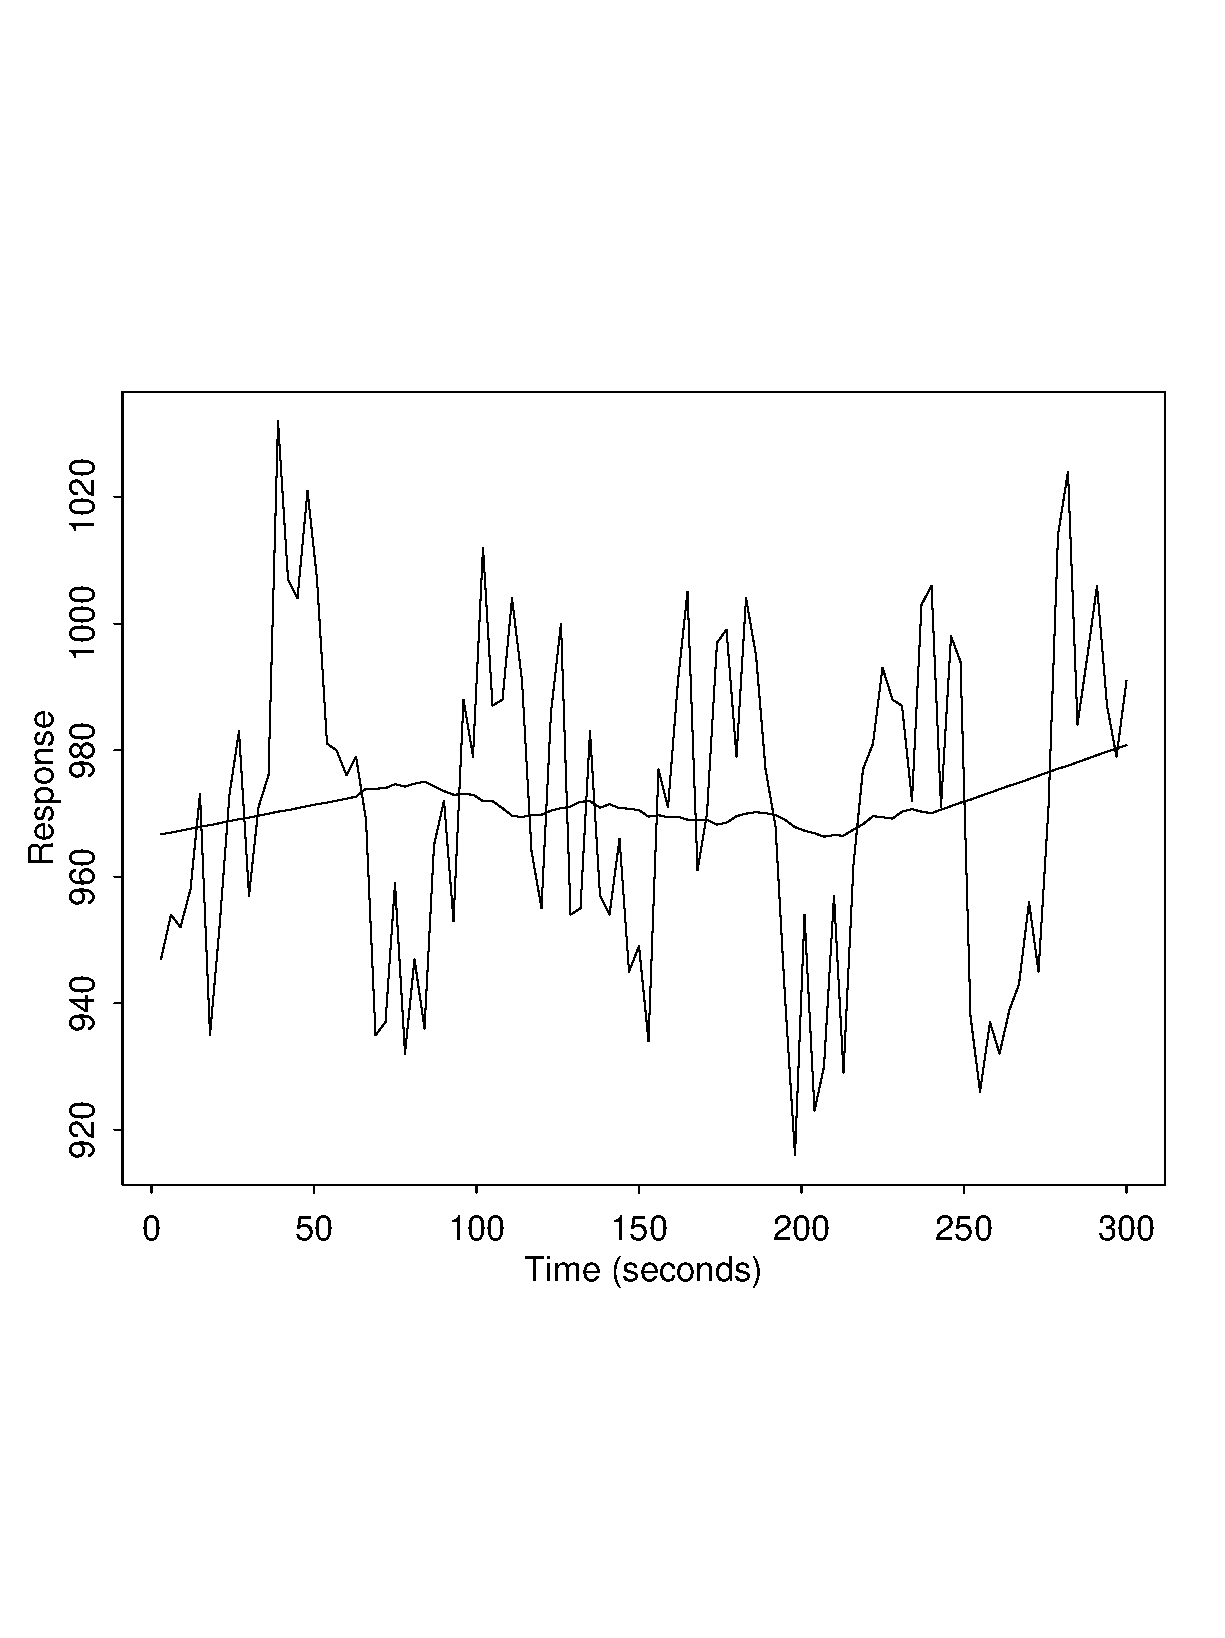
\includegraphics[height=90mm,viewport=25 169 579
    609]{jm_fig2.eps}
  \caption{Trend Removal:(left) Obvious non-linear trend (right) In an area of activation}
\label{trends}
\end{figure}

}
%% Column 2
\col{ 
\paragraph{Theory}
The asymptotic sampling properties of the periodogram are well-known \cite{priestley:1981}.
For increasingly long series:
\begin{itemize}
\item [(I).] $I(\omega_j)/f(\omega_j) \sim \textrm{E}$ where E has a
  standard exponential distribution.
\item [(II).] $I(\omega_j)$ and $I(\omega_k)$ are independent for all
  $k\ne j$.
\end{itemize}
where $f(\omega)$ is the spectral density of the underlying stationary stochastic process.
This is a very general result, includes AR, MA and ARMA processes as special cases and is known to be accurate for series of moderate
length, such as those encountered in fMRI experiments. If we assume that the underlying spectral
density $f(\omega)$ is smooth then we can use a smoothed version of
$I(\omega)$, which we denote $g(\omega)$, to estimate $f(\omega)$.

\paragraph{Estimating the spectral density}
We use a non-parametric estimate of the spectral density and thus avoid the assumptions implicit in parametric approaches. An estimate of the spectral density is obtained by smoothing the
periodogram on log scale \cite{wahba:1980}, $\log(I(\omega))$, to
ensure that the spectral density estimate is positive everywhere. A smoothing spline \cite{silverman:1985} was chosen to
smooth the log-periodogram. The spline is given more freedom at low frequencies to accommodate the effect of the detrending.
To ensure the spectral density of the noise is estimated independently
of any response to the stimulus, the periodogram ordinates at the
fundamental frequency of stimulation and its first two harmonics are
not included in this procedure. Also, a small amount of spatial smoothing is applied to the spectral density estimates. Figure~\ref{periodogram} shows the spectral density estimates before (thick line) and after (dotted line) spatial smoothing.  


\paragraph{Testing for a response to the stimulus}

The spectral density estimate provides us with a baseline against
which to test for significant departures from the underlying process.
From (I),
\begin{equation}
  \frac{I(\omega_j)}{f(\omega_j)} \sim E
\label{eq:13}
\end{equation}
Substituting $g(\omega_j)$ for $f(\omega_j)$, we define the ratio
statistic, $R_j$, as
\begin{equation}
  R_j = \frac{I(\omega_j)}{g(\omega_j)},\qquad\qquad \omega_j=j/\delta
  n
\label{eq:14}
\end{equation}
By calculating the statistic $R_j$ at the fundamental frequency of
activation, $\omega_c$, we obtain a test statistic, $R_c$, for
significant activation. Large values of $R_c$ indicate a large effect at the fundamental
frequency. All of the statistics $R_j$, apart from $j=0$ and $n/2$, will have the same distribution as $R_c$ and thus can be used as a benchmark against which to compare the theoretical distribution of $R_c$, at negligible computational cost. Thus the method is effectively self-calibrating.
}
%% Column 3
\col{
\paragraph{Results}
We have compared our method to an implementation of the AR(1) approach of \cite{Bullmore:1996} in which we apply our own non-linear detrending. Figure~\ref{vis} shows thresholded $p$-value maps of the same slice from a periodic visual stimulation dataset. The AR(1) approach shows significantly more false-positive activation in areas away from the visual cortex. We also applied the two approaches to a null dataset, assuming a periodic stimulus. The distribution of each statistic was compared to its theoretical form using $PP$-plots shown if figure~\ref{pp.plots}. The left plot shows the $PP$-plot of the $R_c$ statistic (thick line) and the $PP$-plot for $R_j$ statistics at a range of higher frequencies (dotted line). The agreement of the dotted line with the theoretical (straight line at $45^o$) validates the use of the theoretical distribution when using our method. For the AR(1) approach shown in the right plot the theoretical is not an adequate fit and a randomisation experiment will be needed to correct for this. 
\paragraph{High frequency artefacts}
In some datasets we have found high frequency artefacts that occur in narrow bands and have been attributed to Nyquist ghosting(figure~\ref{ghost} (right)). We have detected these artefacts using our values of $R_j$ at high frequencies (figure~\ref{ghost} (left) shows a thresholded $R_{88}$ image).
We have found that parametric-time domain models may be extremely susceptible to these artefacts whereas non-parametric spectral density estimation will be resistant. Three methods were applied to a voxel in an area exhibiting the high-frequency artefact. Method I: The AR(1) approach described above, Method II: As Method I but with high frequency artefact removed, Method III: Our approach. Comparing Method I and II, in the table below, we see that the estimated parameters are significantly different after the artefact has been removed, which results in a misleading statistic. Even after removal, there is no guarantee that the AR(1) model is flexible enough and this results in the difference between Methods II and III.
\begin{center}
\small
\begin{tabular}{|l||c|c|c|c|c|}
\hline 
& AR(1) coefficient & $\widehat{\sigma^2}$ & Numerator & Denominator & Ratio Statistic\\
\hline \hline
Method I & $-$0.0027 & 15765 & 591.88 & 315.29 & 1.877\\
\hline
Method II & 0.2839 & 11276 & 624.98 & 419.46 & 1.490\\
\hline 
Method III& --- & --- & 689.30 & 513.88 & 1.341\\
\hline 
\end{tabular}
\end{center}
\paragraph{Conclusion and extensions}
Non-parametric spectral estimation is shown to be an accurate and self-calibrating approach for analyzing periodic designs. The method makes few assumptions and is resistant to high-frequency artefacts whereas parametric time-domain approaches may be susceptible to these artefacts and biased by the assumptions they make on the form of the spectral density. The method can be easily extended to handle non-periodic event related designs and initial results are extremely promising.
\paragraph{Acknowledgements} We are grateful to Dr Stephen Smith (fMRIB Centre, Oxford) for
advice and datasets.

\references
\bibliography{jm.ref}
}
\end{center}


\makefooter

\end{document}





